\documentclass[12pt]{article}
\usepackage[utf8]{inputenc}
\usepackage{amsmath, amssymb}
\usepackage{geometry}
\usepackage{enumitem}
\usepackage{fancyhdr}
\usepackage{booktabs}
\usepackage{longtable}
\usepackage{array}
\usepackage{graphicx}
\usepackage{float}
\usepackage{hyperref}
\usepackage{xcolor}
\geometry{margin=0.75in, top=0.7in, bottom=0.7in}

% Allow URLs to break across lines
\usepackage{url}
\def\UrlBreaks{\do\/\do-\do_\do.\do=\do?\do\&}

\pagestyle{fancy}
\fancyhf{}
\renewcommand{\footrulewidth}{0.4pt}
\fancyfoot[R]{\thepage}

\setlength{\parindent}{0pt}
\setlength{\parskip}{0.2em}

% Compact spacing
\usepackage{enumitem}
\setlist{itemsep=0.05em, topsep=0.05em, leftmargin=1.8em}

\usepackage{titlesec}
\titlespacing*{\section}{0pt}{0.6em}{0.3em}
\titlespacing*{\subsection}{0pt}{0.4em}{0.2em}

\title{DBA5101: Evaluating the RecycleRight Program at NUS}
\author{}
\date{}

\begin{document}

\begin{titlepage}
    \centering
    \vspace*{1cm}
    {\Huge\bfseries DBA5101 Group Project\\[0.5em]}
    {\Huge Evaluating the RecycleRight Program at NUS \par}
    \vspace{1cm}
    
\includegraphics[width=0.30\textwidth]{nus_logo.png} \\[2em]
    {\large Group Members\par}
    \vspace{0.5cm}
    {\small
    CHAN HIU LOK \\[0.2em]
    CHEN HANGYU \\[0.2em]
    SANYA RAJPAL \\[0.2em]
    TANYA TOOLEY \\[0.2em]
    WANG YING \\[0.2em]
    }
    \vspace{1cm}
    {\large
    National University of Singapore \\
    \vspace{0.5cm}
    Submission Date: October 11, 2025 \\
    \vspace{0.3cm}
    \href{https://github.com/ying-jeanne/managerial_economics}{Link to code repository}
    }
    \vfill
\end{titlepage}
\thispagestyle{fancy}

\section{Introduction \& Defining the Problem}

\textbf{Objective:} Evaluate the causal impact of shaped bin openings (Phase 2) and informational banners (Phase 3) on contamination of paper, plastic, and cans at NUS.

\textbf{Problem:} High contamination increases waste management costs and lowers the value of recyclables.

\textbf{Research Questions:}
\begin{enumerate}
    \item Do shaped openings reduce contamination?
    \item Do informational banners provide additional improvement?
    \item Which intervention is more effective for each material type?
\end{enumerate}

\section{Understanding the Experimental Design}

This project employs a quasi-experimental design that is well-suited for a \textbf{Difference-in-Differences (DiD)} analysis. This method allows us to isolate the true effect of the interventions from other time-based trends.

\textbf{Treatment Group (UTOWN):} Sequential interventions
\begin{itemize}
    \item Phase 1: Baseline (standard bins)
    \item Phase 2: Shaped openings
    \item Phase 3: Shaped openings + banners
\end{itemize}

\textbf{Control Group (ENGINE):} Standard bins throughout, providing a counterfactual.

\textbf{Key Metrics:} PaperContaminant, PlasticContaminant, CanContaminant.

\section{Data Exploration and Preparation}

\subsection{Data Cleaning and Anomalous Data Point Removal}

The raw dataset initially contained 255 rows, with 170 being empty formatting artifacts (where Area = NaN), which were subsequently removed. Following this, two observations on 2020-02-02 (one per location) were identified with suspicious 0.0\% contamination values for paper and plastic, and missing data for cans. Analysis of neighboring dates (see \hyperref[tab:feb2]{Table A1} in Appendix) revealed typical contamination rates between 1\% and 65\%, indicating that 0.0\% was a statistical impossibility and likely a systematic data collection failure.

Both observations for 2020-02-02 were removed. This removal does not bias our Difference-in-Differences (DiD) estimates as it was balanced across both treatment and control groups and preserves parallel trends.

\subsection{Ensuring Balanced Structure for DiD Validity}

A critical requirement for a valid Difference-in-Differences analysis is that both the treatment (UTOWN) and control (ENGINE) groups have observations on the same dates. To ensure this balanced panel structure, five unbalanced dates were identified and removed: three ENGINE-only dates (2020-01-16, 2020-02-07, 2020-03-10) and two UTOWN-only dates (2020-01-13, 2020-01-14). While this reduced the sample size, maintaining a balanced panel is non-negotiable for credibly attributing post-intervention changes to the treatment effect.

\subsection{Exploratory Data Analysis (EDA)}

After cleaning and balancing, the final dataset comprised 78 observations (39 per location) spanning Phase 1 (Baseline: Jan 15 -- Feb 10), Phase 2 (Shaped Openings: Feb 11 -- Feb 22), and Phase 3 (Shaped Openings + Banners: Mar 4 -- Mar 17).

\textbf{Key Observations from Summary Statistics (see \hyperref[tab:paper]{Tables A2}-\hyperref[tab:cans]{A4} in Appendix):}

\begin{itemize}
    \item \textbf{Baseline Contamination Levels (Phase 1):} UTOWN consistently exhibited significantly higher contamination rates than ENGINE across all materials (Paper: 6.10\% vs 0.87\%; Plastic: 59.73\% vs 49.04\%; Cans: 35.47\% vs 13.77\%). This highlights the necessity of the DiD approach to control for these persistent pre-existing differences.

    \item \textbf{Plastic Shows Campus-Wide Time Trend:} Both ENGINE and UTOWN experienced substantial, nearly identical decreases in plastic contamination from Phase 1 to Phase 2 ($\approx$13 pp). This suggests a campus-wide time trend, such as seasonal changes or broader awareness campaigns, unrelated to the shaped-opening intervention.

    \item \textbf{Can Contamination Shows Largest Changes:} UTOWN's can contamination dramatically dropped by 48\% in Phase 2 (35.47\% $\rightarrow$ 18.34\%), while ENGINE remained relatively stable. This preliminary observation points towards a potential treatment effect for cans.

    \item \textbf{Phase 3 Plastic Reversal:} UTOWN's plastic contamination sharply rebounded in Phase 3 (46.51\% $\rightarrow$ 59.18\%), nearly returning to baseline, suggesting a potential adverse effect of informational banners.
\end{itemize}

\subsection{Parallel Trends Assessment (Critical for DiD Validity)}

The validity of our Difference-in-Differences analysis hinges on the parallel trends assumption, meaning the treatment and control groups would have followed similar trends in the absence of intervention. Both visual inspection of time-series line charts (see \hyperref[fig:parallel_trends]{Figure A1} in Appendix) and formal statistical tests confirmed this assumption for all three materials during Phase 1. The interaction coefficient in regressions of Phase 1 contamination rates on time, treatment, and their interaction was not statistically significant for paper ($p > 0.05$), plastic ($p > 0.05$), or cans ($p > 0.05$). This robust evidence validates our DiD approach, allowing us to credibly attribute post-intervention divergences to causal treatment effects.

\section{Statistical Analysis: Difference in Differences (DiD)}

Difference-in-Differences (DiD) is a quasi-experimental method that isolates the causal effect of an intervention by comparing the change in the treatment group to the change in the control group over the same period. This approach effectively controls for time-invariant differences between groups and common time trends affecting both groups. The core DiD logic is:

\begin{equation}
\text{DiD\_Effect} = (\text{UTOWN}_{\text{after}} - \text{UTOWN}_{\text{before}}) - (\text{ENGINE}_{\text{after}} - \text{ENGINE}_{\text{before}})
\end{equation}

We conducted two separate DiD analyses using linear regression models to evaluate each intervention, providing robust statistical inference. The general regression model used was:

\begin{equation}
\text{Contamination} = \beta_0 + \beta_1 \cdot \text{PostPhase} + \beta_2 \cdot \text{IsUTOWN} + \delta \cdot (\text{PostPhase} \times \text{IsUTOWN}) + \varepsilon
\end{equation}

Where $\delta$ (the interaction term) represents the DiD estimator, which is the causal effect of the intervention.

\subsection{Phase 2 Analysis: Shaped Openings Effect}

\textbf{Research Question:} Did shaped bin openings reduce contamination rates at UTOWN relative to ENGINE?

\textbf{Comparison Periods:}
\begin{itemize}
    \item Before: Phase 1 (baseline, January 15 - February 10)
    \item After: Phase 2 (shaped openings introduced, February 11 - February 22)
    \item Sample: 56 observations (28 per location)
\end{itemize}

\textbf{Hypotheses:}
\begin{itemize}
    \item $H_0$: $\delta_1 = 0$ (shaped openings had no effect)
    \item $H_1$: $\delta_1 \neq 0$ (shaped openings affected contamination)
\end{itemize}

\textbf{Results (see \hyperref[tab:phase2]{Table A5} in Appendix for full details):}

\begin{itemize}
    \item \textbf{Cans (Highly Significant):} Shaped openings caused a substantial 15.02 percentage point reduction in can contamination at UTOWN ($p = 0.007$), representing a 43\% decrease from the baseline rate. This effect is highly statistically significant and practically meaningful.

    \item \textbf{Paper (Marginally Significant):} Shaped openings reduced paper contamination by 2.52 percentage points ($p = 0.048$), a 41\% decrease from baseline. This effect is statistically significant at the 5\% level.

    \item \textbf{Plastic (Not Significant):} Shaped openings had no statistically significant effect on plastic contamination ($p = 0.978$). The DiD approach successfully controlled for a campus-wide time trend, where both ENGINE and UTOWN experienced similar decreases ($\approx$13 pp) during this period, unrelated to the intervention.

    \item \textbf{Key Insight:} Physical design cues (shaped openings) effectively reduced contamination for cans and paper but had no significant effect on plastic recycling.
\end{itemize}

\subsection{Phase 3 Analysis: Informational Banners Effect}

\textbf{Research Question:} Did adding informational banners provide additional benefit beyond shaped openings alone?

\textbf{Comparison Periods:}
\begin{itemize}
    \item Before: Phase 2 (shaped openings only, February 11 - February 22)
    \item After: Phase 3 (shaped openings + banners, March 4 - March 17)
    \item Sample: 44 observations (22 per location)
\end{itemize}

\textbf{Hypotheses:}
\begin{itemize}
    \item $H_0$: $\delta_2 = 0$ (banners had no additional effect)
    \item $H_1$: $\delta_2 < 0$ (banners provided additional contamination reduction)
\end{itemize}

\textbf{Results (see \hyperref[tab:phase3]{Table A6} in Appendix for full details):}

\begin{itemize}
    \item \textbf{Plastic (Significant Adverse Effect):} Contrary to expectations, informational banners significantly increased plastic contamination by 9.24 percentage points ($p = 0.038$). This backfire effect erased most of the Phase 2 improvements, returning contamination nearly to baseline levels, indicating harm rather than benefit.

    \item \textbf{Paper and Cans (Not Significant):} Banners showed no statistically significant additional effects for paper ($p = 0.240$) or cans ($p = 0.139$). However, the positive point estimates suggest potential harm rather than benefit, though a zero effect cannot be ruled out.

    \item \textbf{Key Insight:} Adding informational banners not only failed to improve recycling behavior but actually worsened plastic contamination, suggesting information overload, confusion, or distraction from the effective physical design cues of Phase 2.
\end{itemize}

\subsection{Summary of Causal Effects}

See \hyperref[tab:summary]{Table A7} in Appendix for a complete summary of all DiD treatment effects.

\textbf{Overall Conclusion:} Shaped bin openings are an effective intervention for reducing can and paper contamination (15.02 pp and 2.52 pp reductions respectively, both statistically significant), but informational banners backfired for plastic recycling (+9.24 pp increase, $p = 0.038$). Physical design cues outperform informational messaging for guiding recycling behavior.

\section{Synthesizing Results and Discussion}

Our Difference-in-Differences (DiD) analyses revealed distinct causal impacts of shaped bin openings (Phase 2) and informational banners (Phase 3) on recycling contamination rates for paper, plastic, and cans. The credibility of these DiD estimates is strongly supported by both visual inspection and statistical tests confirming parallel trends between the treatment (UTOWN) and control (ENGINE) groups during the baseline period.

\textbf{Key Findings:}

\begin{itemize}
    \item \textbf{Shaped Openings (Phase 2):}
    \begin{itemize}
        \item \textbf{Cans:} Highly significant 15.02 percentage point reduction ($p = 0.007$), representing a 43\% decrease from baseline.
        \item \textbf{Paper:} Marginally significant 2.52 percentage point reduction ($p = 0.048$), a 41\% decrease from baseline.
        \item \textbf{Plastic:} No statistically significant effect ($p = 0.978$). A campus-wide time trend ($\approx$13 pp decrease in both groups) was observed, which the DiD approach successfully controlled for.
    \end{itemize}

    \item \textbf{Informational Banners (Phase 3):}
    \begin{itemize}
        \item \textbf{Plastic:} Significantly increased contamination by 9.24 percentage points ($p = 0.038$), erasing most Phase 2 improvements.
        \item \textbf{Paper and Cans:} No statistically significant additional effects. Positive (though non-significant) point estimates suggest potential harm rather than benefit.
    \end{itemize}
\end{itemize}

See \hyperref[tab:summary]{Table A7} in Appendix for a complete summary of all DiD treatment effects.

\section{Managerial Recommendations}

This section builds on our statistical findings to explain why Phase 2 (shaped openings) works while Phase 3 (banners) does not, and to recommend what to scale. We unpack the behavioral mechanisms underlying our results, triangulate with global evidence of interventions that have measurably improved recycling purity, and present a defensible business case for campus-wide implementation. The goal is actionable guidance for rolling out shaped-opening bins for paper and cans, adopting RecycleRight-style ``at-hand'' features for plastics, and retiring overhead banners---interventions that reduce contamination, improve recyclate value, and future-proof operations against tightening waste regulations.

\subsection{Behavioral mechanisms: Why shaped openings work but banners don't}

At bins, decisions are fast, habitual, and attention-poor. Shaped openings function as poka-yoke affordances: a slot implies flat paper, a circular aperture implies a can, and a short guided chute invites the bottle in the correct orientation. These cues interrupt the toss just enough to convert an automatic move into a correct one---without demanding reading or memory. Banners, by contrast, require visual search and comprehension away from the motor action, they tend to be largely ignored and they compete with habit and time pressure (Tan et al., 2024), so they are filtered out. Where plastic improved was precisely when the design changed the deposit choreography and removed back-of-house pain like having front pull out doors reducing error-prone workarounds (Zelenika et al., 2018). In other words, Phase 2 touched the hand, and Phase 3 tried to teach the head. Behaviour follows the former (Phase 2). The RecyleRight design also reduced cleaner strain by replacing vertical lifts with front pull-out doors---a critical operational win often overlooked in bin design.

\subsection{Global evidence and what to borrow next}

\textbf{With human-centred design and operations.} Cities that add direct feedback at the cart-inspection plus ``oops'' tags, consistently drive down contamination. Grand Rapids' Feet-on-the-Street campaign cut contamination by 37\% in a single season and has since embedded truck mounted cameras to sustain quality. In event and cafeteria settings, on-site station helpers virtually eliminate mistakes: a controlled study found $\approx$96--97\% contamination reductions in staffed conditions. Well-placed, eye level signs and simple ``yes/no'' labels at the opening help when they're at the point of action and not overhead banners. Together, these cases validate NUS's core insight: intervene where the hand is, and give immediate, specific feedback (Heffernan, 2022; The Recycling Partnership, 2025; Oregon Department of Environmental Quality [Oregon DEQ], 2024; Zelenika et al., 2018).

\textbf{Governance and system design-wise,} system levers create purity at scale. Dual-stream collection---separating fibres from containers has taken cities from $\sim$20\% contamination down to $\sim$5--7\%, as documented in Lake Worth Beach and others (Waste Dive, 2018; City of Mission, 2025), with outreach to help residents re-learn the split. Producer-led EPR programs enforce tight contamination caps; Recycle BC (2025) sets thresholds around 5\% and cities like Mission, BC have cut contamination by $>$40\% to stay under the cap. Deposit-return systems push beverage containers into a separate, near-contamination-free stream with return rates often above 90\%, supplying high-grade material back to producers. These tools don't replace human-centred design at bins; they complement it by aligning incentives and standards across the system (Recycle BC, 2025; TOMRA, n.d.). This approach not only improved recycling purity but also lowers servicing time, reduces rejected loads, and enhances compliance readiness, delivering tangible ROI across operational, environmental, and reputational dimensions.

\subsection{What to scale now}

To reduce recycling contamination, NUS should consider scale-shaped opening bins for paper and cans, retire overhead banners, and deploy RecycleRight-style, at-hand features for plastics campus-wide. This combination maps to how people actually behave (fast, habitual), preserves throughput, reduces cleaner workarounds, and aligns with global best practice that couples choice architecture with immediate feedback. This also underpins a credible ROI narrative, lower contamination and fewer rejected loads, higher recyclate value, and faster, safer servicing---while remaining compatible with future governance levers should Singapore move toward tighter contamination standards or deposit models.

\newpage
\appendix

\section{Appendix: Supporting Tables and Figures}

\begin{figure}[H]
\centering
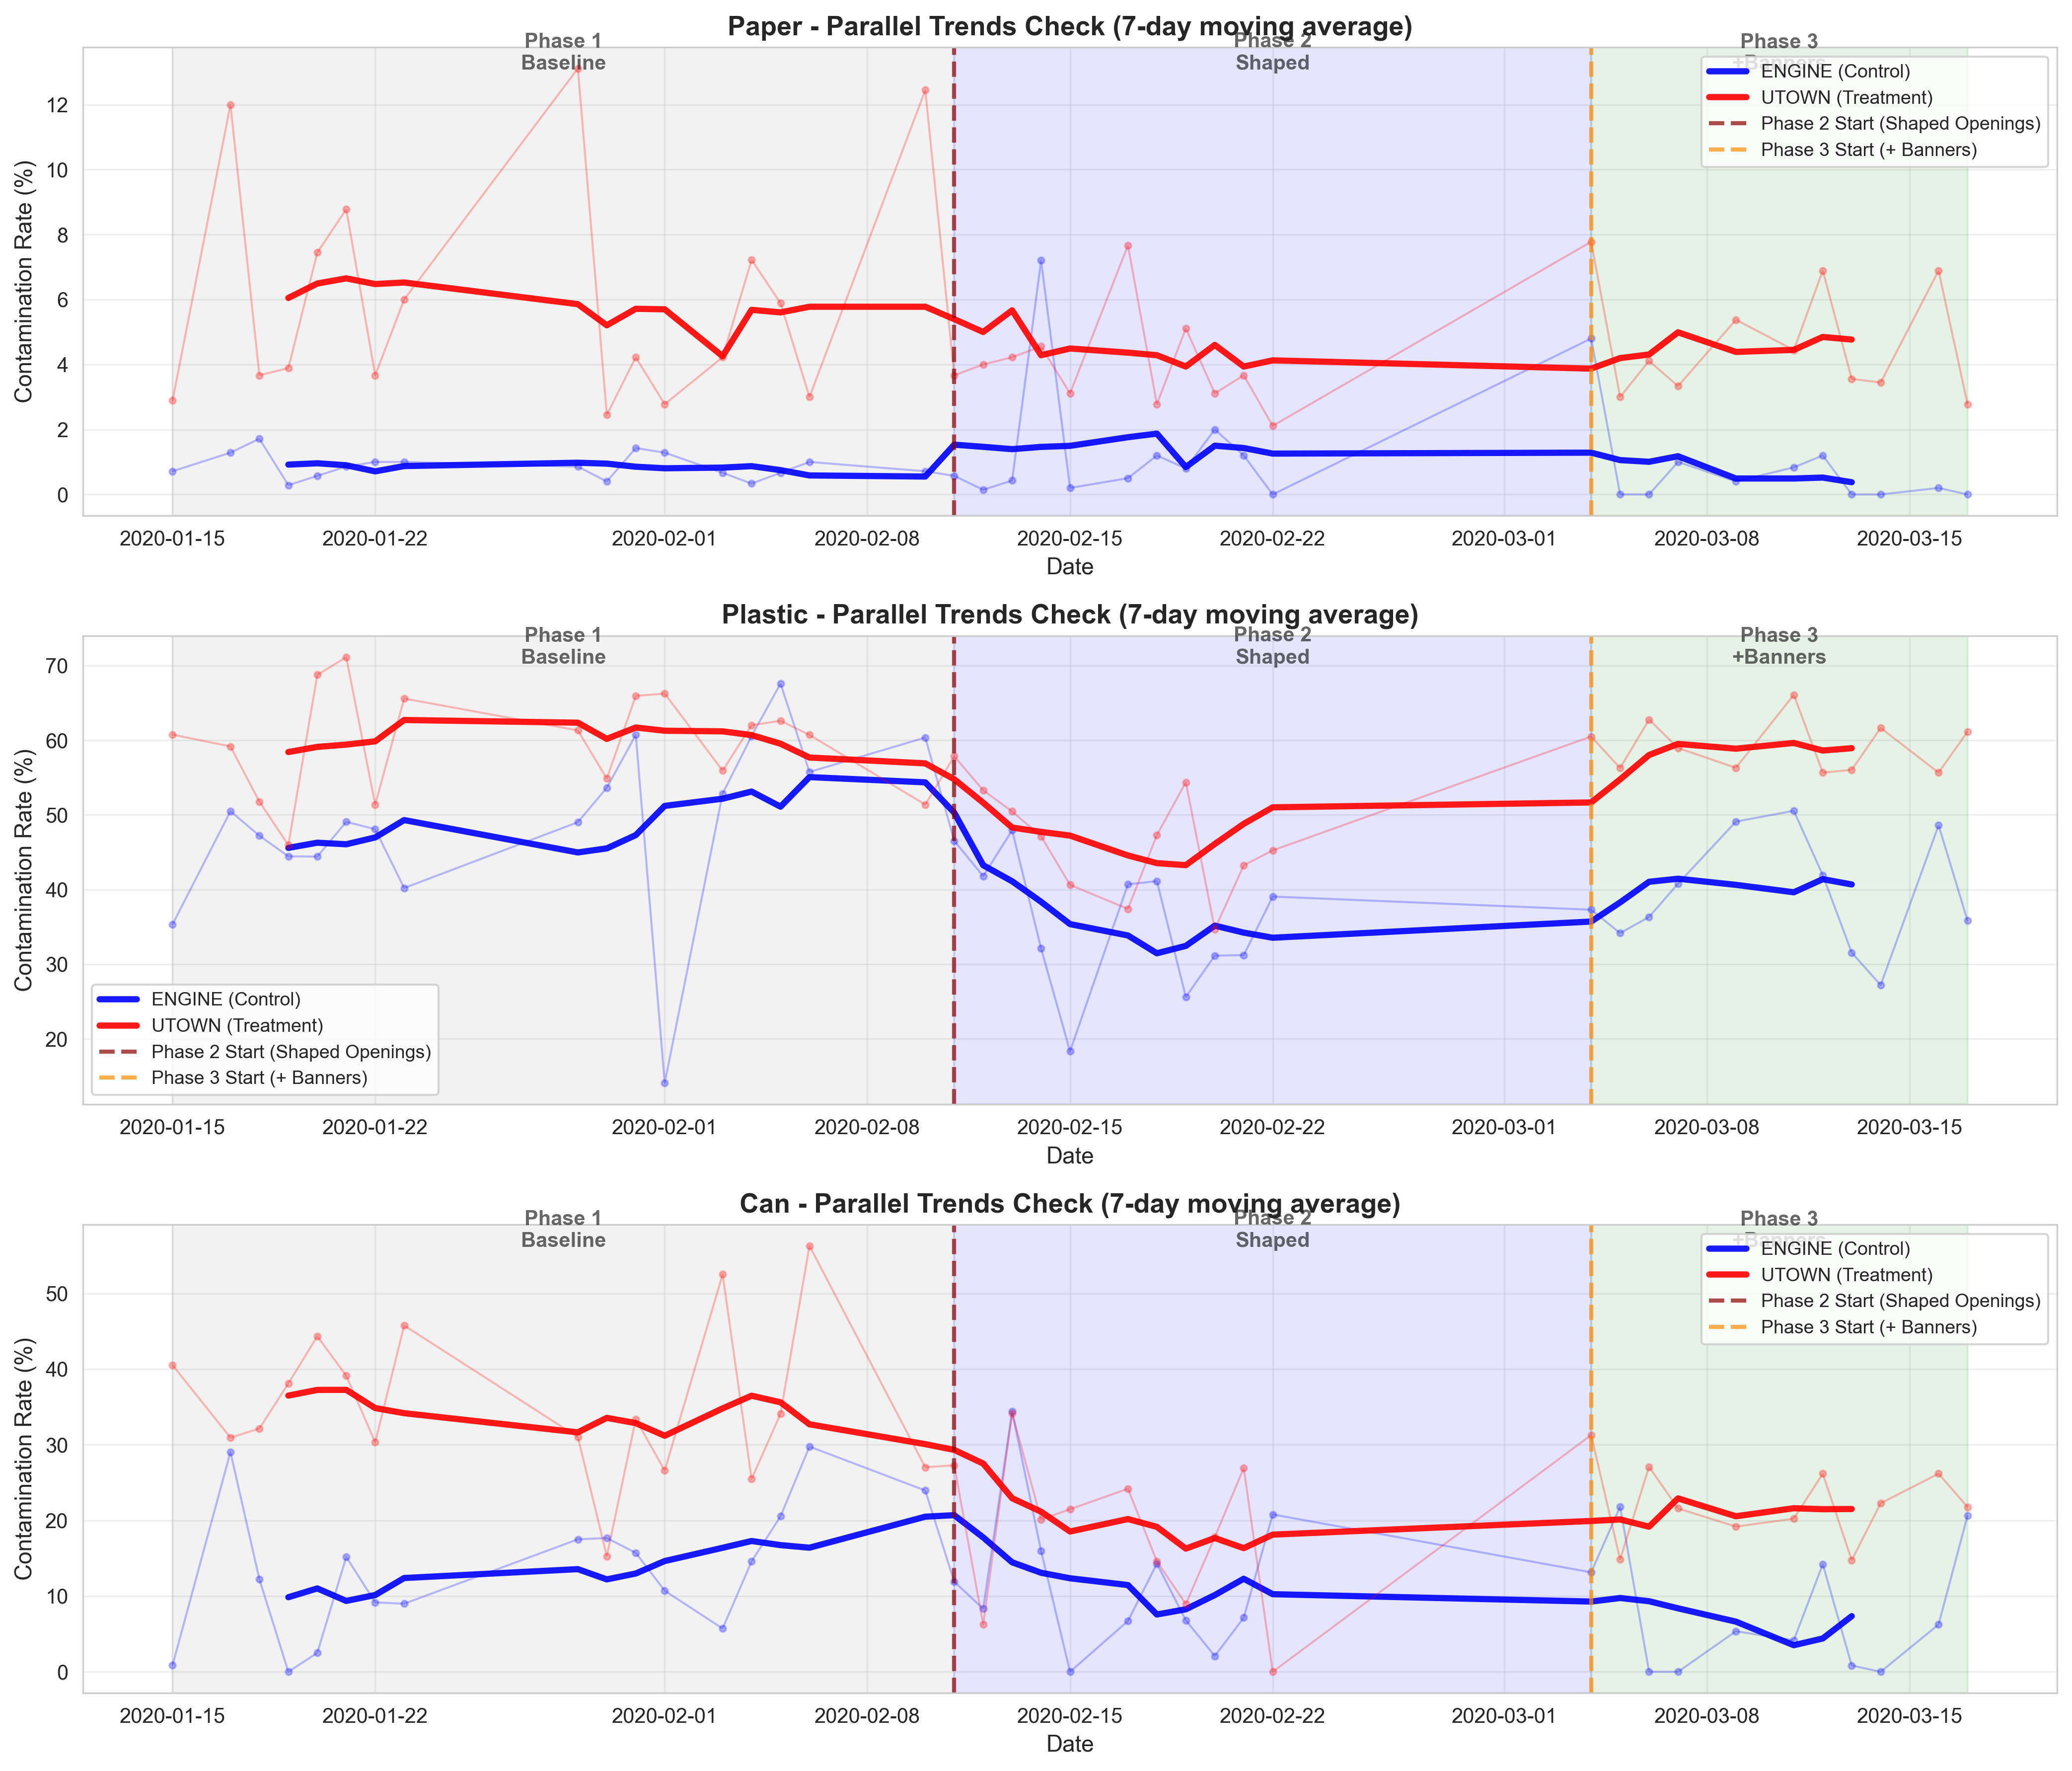
\includegraphics[width=\textwidth]{parallel_trends_check.png}
\caption{Parallel Trends Check -- Contamination Rates Over Time}
\label{fig:parallel_trends}
\end{figure}

\begin{table}[H]
\centering
\caption{Contamination rates from 2020-01-30 to 2020-02-05}
\label{tab:feb2}
\small
\begin{tabular}{lrrrrrr}
\toprule
& \multicolumn{2}{c}{Paper (\%)} & \multicolumn{2}{c}{Plastic (\%)} & \multicolumn{2}{c}{Cans (\%)} \\
\cmidrule(lr){2-3} \cmidrule(lr){4-5} \cmidrule(lr){6-7}
Date & ENGINE & UTOWN & ENGINE & UTOWN & ENGINE & UTOWN \\
\midrule
2020-01-30 & 0.40 & 2.44 & 53.63 & 54.86 & 17.68 & 15.27 \\
2020-01-31 & 1.43 & 4.22 & 60.71 & 65.94 & 15.71 & 33.38 \\
2020-02-01 & 1.29 & 2.78 & 14.07 & 66.24 & 10.71 & 26.59 \\
\textbf{2020-02-02} & \textbf{0.00} & \textbf{0.00} & \textbf{0.00} & \textbf{0.00} & \textbf{---} & \textbf{---} \\
2020-02-03 & 0.67 & 4.22 & 52.84 & 55.93 & 5.71 & 52.53 \\
2020-02-04 & 0.33 & 7.22 & 60.56 & 62.01 & 14.58 & 25.46 \\
2020-02-05 & 0.67 & 5.89 & 67.58 & 62.60 & 20.54 & 34.09 \\
\bottomrule
\end{tabular}
\end{table}

% \begin{figure}[H]
% \centering
% 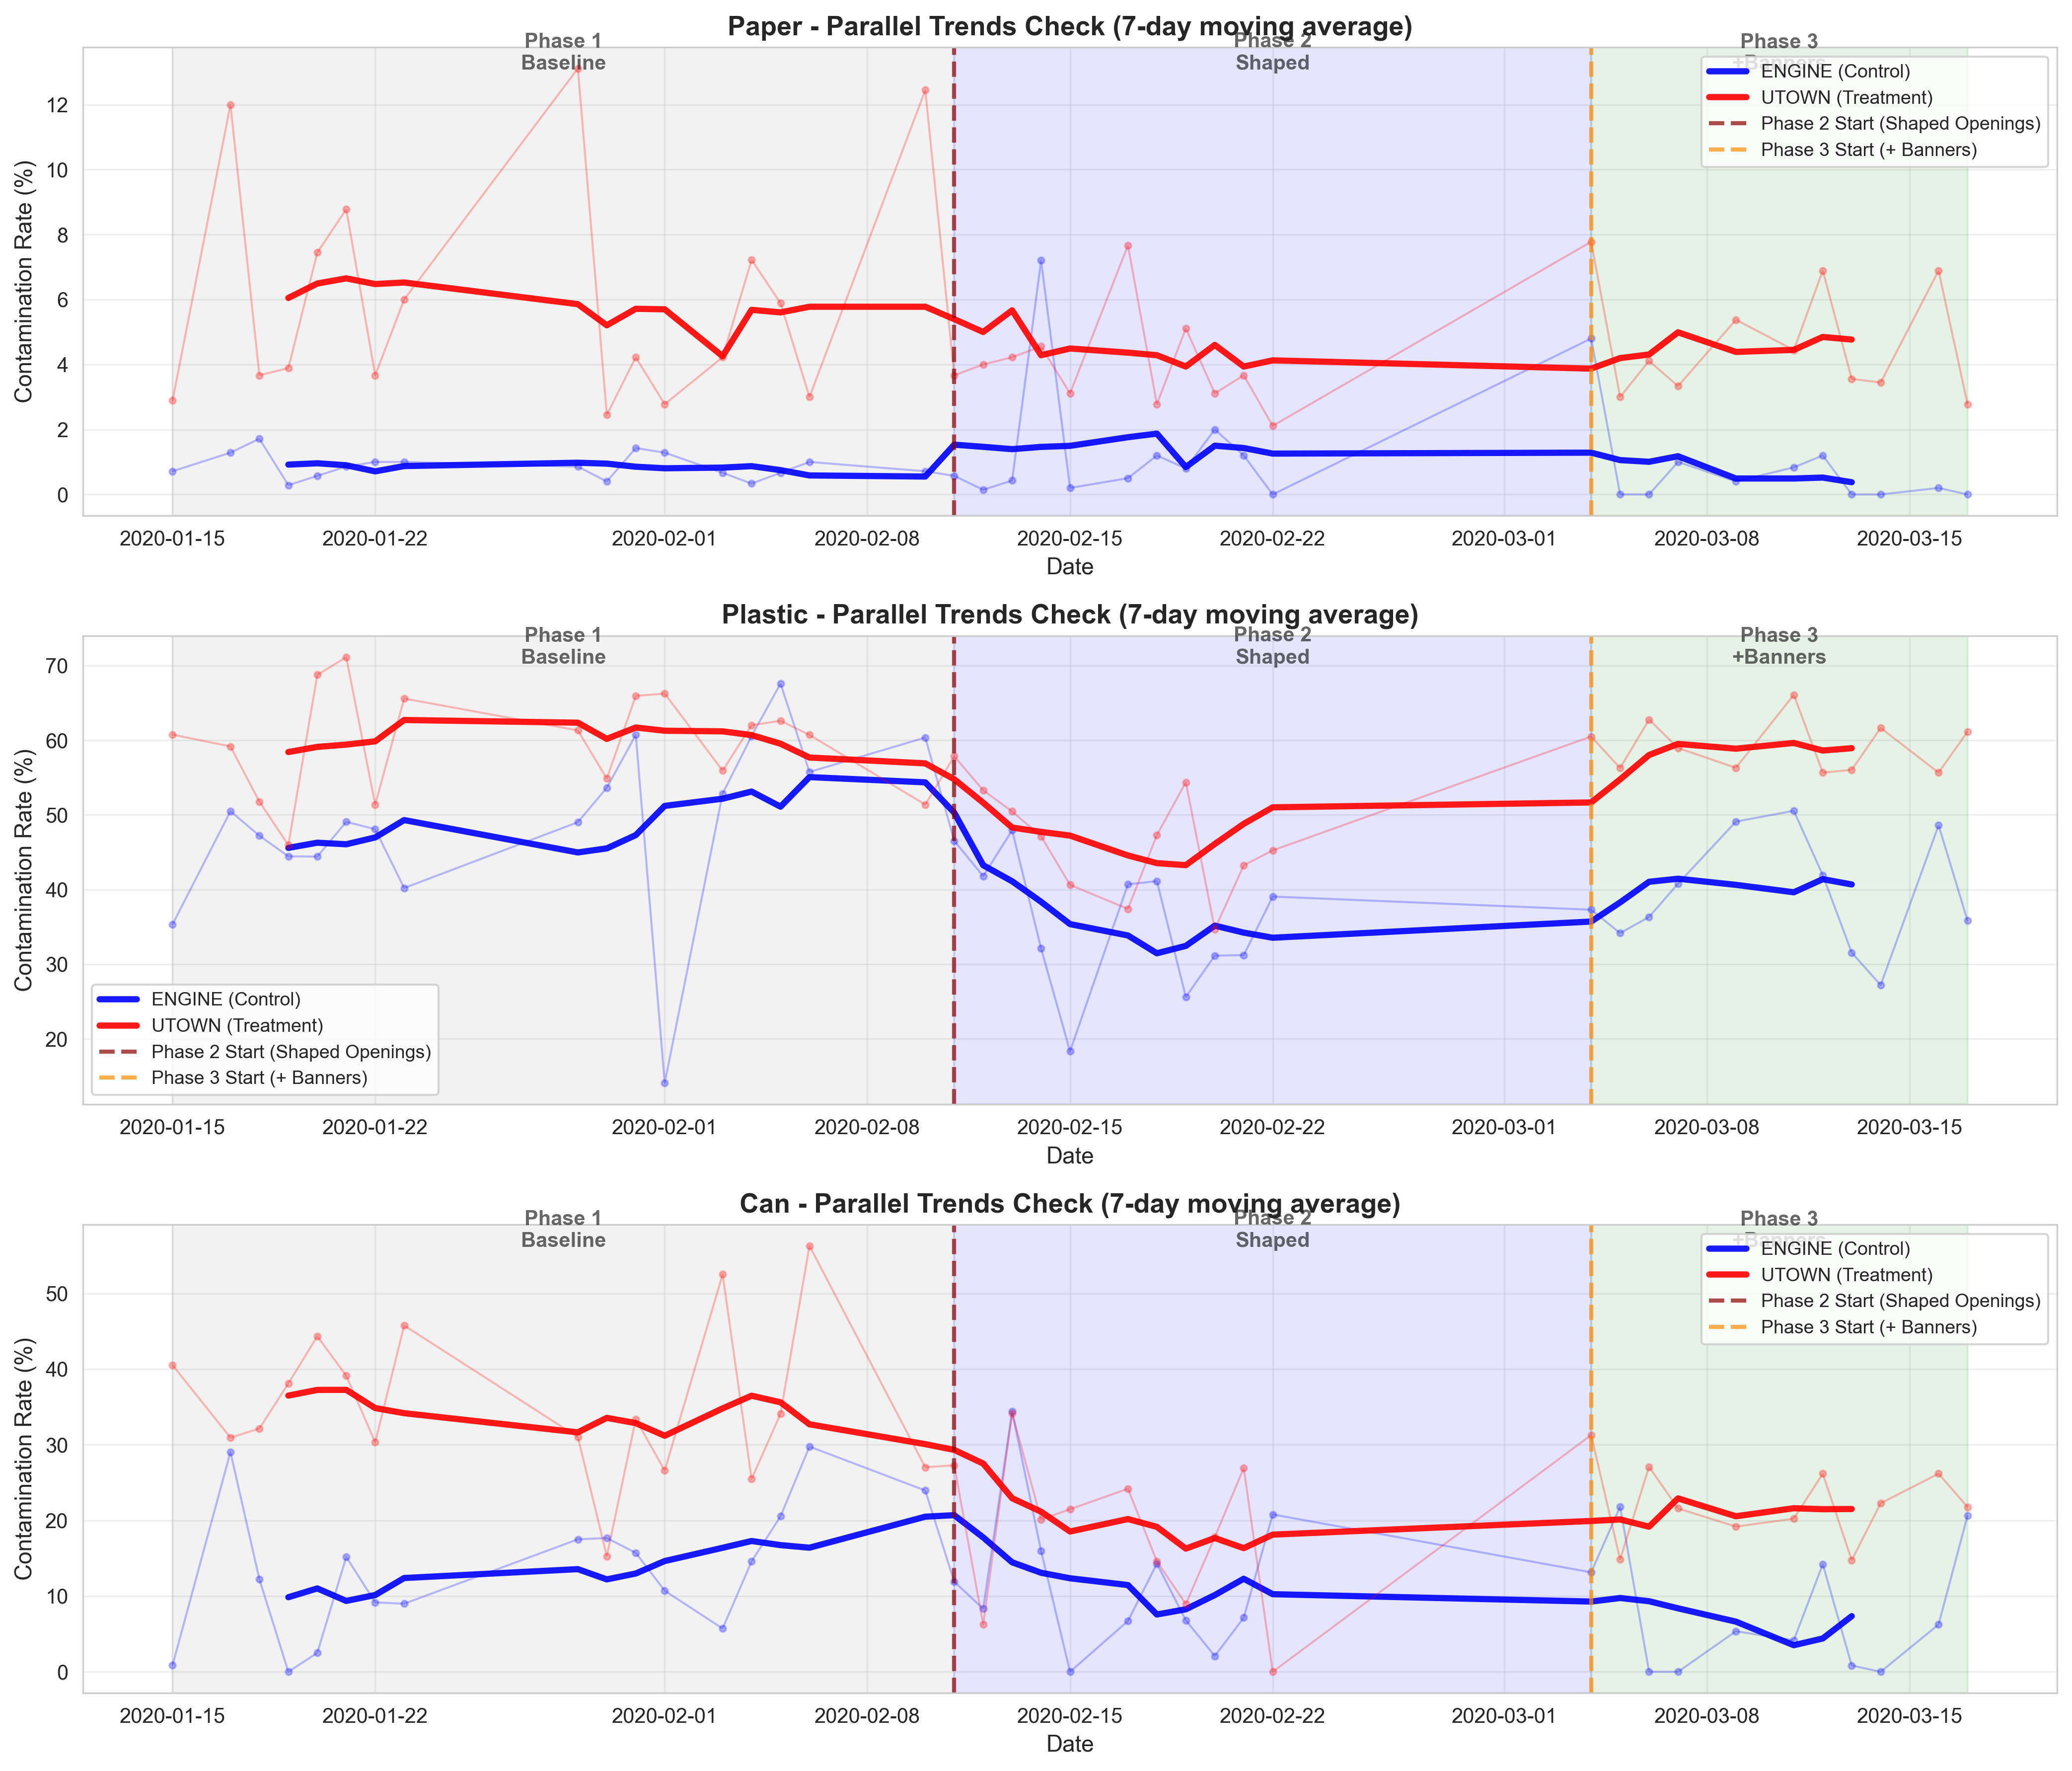
\includegraphics[width=\textwidth]{parallel_trends_check.png}
% \caption{Parallel Trends Check -- Contamination Rates Over Time}
% \end{figure}

\begin{table}[H]
\centering
\caption{Paper Contamination Summary Statistics (\%)}
\label{tab:paper}
\small
\begin{tabular}{llrrrrrr}
\toprule
Phase & Location & Datapoints(N) & Mean & Median & Std Dev & Min & Max \\
\midrule
1 & ENGINE & 17 & 0.87 & 0.86 & 0.39 & 0.29 & 1.71 \\
1 & UTOWN & 17 & 6.10 & 4.22 & 3.56 & 2.44 & 13.11 \\
2 & ENGINE & 11 & 1.29 & 0.57 & 2.04 & 0.00 & 7.20 \\
2 & UTOWN & 11 & 4.00 & 3.67 & 1.48 & 2.11 & 7.67 \\
3 & ENGINE & 11 & 0.77 & 0.20 & 1.41 & 0.00 & 4.80 \\
3 & UTOWN & 11 & 4.69 & 4.11 & 1.77 & 2.78 & 7.78 \\
\bottomrule
\end{tabular}
\end{table}

\begin{table}[H]
\centering
\caption{Plastic Contamination Summary Statistics (\%)}
\label{tab:plastic}
\small
\begin{tabular}{llrrrrrr}
\toprule
Phase & Location & Datapoints(N) & Mean & Median & Std Dev & Min & Max \\
\midrule
1 & ENGINE & 17 & 49.04 & 49.07 & 12.14 & 14.07 & 67.58 \\
1 & UTOWN & 17 & 59.73 & 60.75 & 6.96 & 45.96 & 71.12 \\
2 & ENGINE & 11 & 35.96 & 39.06 & 9.09 & 18.33 & 47.93 \\
2 & UTOWN & 11 & 46.51 & 47.13 & 7.23 & 34.68 & 57.85 \\
3 & ENGINE & 11 & 39.39 & 37.29 & 7.59 & 27.21 & 50.54 \\
3 & UTOWN & 11 & 59.18 & 58.96 & 3.52 & 55.66 & 66.08 \\
\bottomrule
\end{tabular}
\end{table}

\begin{table}[H]
\centering
\caption{Can Contamination Summary Statistics (\%)}
\label{tab:cans}
\small
\begin{tabular}{llrrrrrr}
\toprule
Phase & Location & Datapoints(N) & Mean & Median & Std Dev & Min & Max \\
\midrule
1 & ENGINE & 17 & 13.77 & 14.58 & 8.94 & 0.00 & 29.76 \\
1 & UTOWN & 17 & 35.47 & 33.38 & 10.30 & 15.27 & 56.28 \\
2 & ENGINE & 11 & 11.67 & 8.33 & 9.66 & 0.00 & 34.40 \\
2 & UTOWN & 11 & 18.34 & 20.14 & 10.18 & 0.00 & 34.17 \\
3 & ENGINE & 11 & 7.86 & 5.36 & 8.27 & 0.00 & 21.81 \\
3 & UTOWN & 11 & 22.31 & 21.77 & 5.11 & 14.75 & 31.28 \\
\bottomrule
\end{tabular}
\end{table}

\begin{table}[H]
\centering
\caption{Phase 2 DiD Results (Shaped Openings Effect)}
\label{tab:phase2}
\small
\begin{tabular}{lrrrll}
\toprule
Material & DiD Estimate ($\delta_1$) & Std Error & p-value & 95\% CI & Significant? \\
\midrule
Paper & $-2.52$ pp & 1.24 & 0.048 & [$-5.02$, $-0.03$] & Yes \\
Plastic & $-0.14$ pp & 5.08 & 0.978 & [$-10.33$, $10.06$] & No \\
Cans & $-15.02$ pp & 5.34 & 0.007 & [$-25.73$, $-4.32$] & Yes \\
\bottomrule
\end{tabular}
\end{table}

\begin{table}[H]
\centering
\caption{Phase 3 DiD Results (Banner Effect)}
\label{tab:phase3}
\small
\begin{tabular}{lrrrll}
\toprule
Material & DiD Estimate ($\delta_2$) & Std Error & p-value & 95\% CI & Significant? \\
\midrule
Paper & $+1.22$ pp & 1.02 & 0.240 & [$-0.85$, $3.28$] & No \\
Plastic & $+9.24$ pp & 4.31 & 0.038 & [$+0.52$, $+17.96$] & Yes (adverse) \\
Cans & $+7.78$ pp & 5.15 & 0.139 & [$-2.62$, $+18.18$] & No \\
\bottomrule
\end{tabular}
\end{table}

\begin{table}[H]
\centering
\caption{Summary of DiD Treatment Effects}
\label{tab:summary}
\small
\begin{tabular}{lccc}
\toprule
Intervention & Paper & Plastic & Cans \\
\midrule
\textbf{Shaped Openings (Phase 2)} & \checkmark $-2.52$ pp* (41\% $\downarrow$) & $\times$ No effect & \checkmark $-15.02$ pp** (43\% $\downarrow$) \\
\textbf{Banners (Phase 3)} & $\times$ No effect & \textcolor{red}{$\bigtriangleup$ $+9.24$ pp* (backfire)} & $\times$ No effect \\
\bottomrule
\multicolumn{4}{l}{\small *$p < 0.05$, **$p < 0.01$}
\end{tabular}
\end{table}

\newpage
\section*{References}

\raggedright
\setlength{\parskip}{0.5em}

\textbf{Grand Rapids -- The Recycling Partnership.} (2025, September 22). Catalyzing recycling system change in Grand Rapids, Michigan. \\
\url{https://recyclingpartnership.org/system-change-grand-rapids-michigan-impact-story/}

\textbf{Heffernan, M.} (2021, August 24). Cart tags: A growing force in fight against contamination. \textit{Resource Recycling}. \\
\url{https://resource-recycling.com/recycling/2021/08/24/cart-tags-a-growing-force-in-fight-against-contamination/}

\textbf{City of Mission.} (2025, March 25). Residents significantly reduce contamination in recycling. \\
\url{https://www.mission.ca/council-government/news/residents-significantly-reduce-contamination-recycling}

\textbf{Recycle BC.} (2025, June 6). 2024 Annual report (contamination threshold policy update). \\
\url{https://recyclebc.ca/wp-content/uploads/2025/06/Recycle-BC_Annual-Report_2024_F.pdf}

\textbf{TOMRA.} (2025, August 18). What is a bottle bill? Retrieved from TOMRA Reverse Vending. \\
\url{https://www.tomra.com/reverse-vending/media-center/feature-articles/what-is-a-bottle-bill}

\textbf{TOMRA.} (n.d.). Deposit return schemes FAQ (separate collection prevents contamination). Retrieved October 14, 2025. \\
\url{https://www.tomra.com/reverse-vending/deposit-return-schemes-faq}

\textbf{Waste Dive.} (2018, September 4). Lake Worth, Florida reverting to dual-stream collection; single-stream contamination about 39\%. \\
\url{https://www.wastedive.com/news/lake-worth-florida-dual-stream-collection/531504/}

\textbf{Recycling Today.} (2019, May 23). Taking sides on single- or dual-stream recycling (contamination down to 5--7\%). \\
\url{https://www.recyclingtoday.com/news/wasteexpo-2019-dual-stream-vs-single-stream/}

\textbf{Tan, H. M., Too, K. A., Lin, D., \& Goh, J.} (2024). Toward Zero Waste: RecycleRight at the National University of Singapore (Ivey case W37339). Ivey Publishing

\end{document}
